% !TEX root =  ../main.tex
\section{Approach}
\label{sec:approach}


In this section, we provide an overview of our approach for automatically generating exploits as proofs of application vulnerabilities.

\subsection{Problem Formulation and Approach Overview} We formulate the problem as follows. Let the \textit{state} of an application at a particular point in the program be defined as a set of (variable, value) pairs $V = \{(v_1, a_1), (v_2, a_2), ...,$ \\
$ (v_n, a_n)\}$ visible at that point during execution. 
% Obviously, for every point in the program, there can be many possible states during execution. These states depend on the variable values at the \textit{source} statements, on the paths from those statements to the program points, and on the operations over the variable values along those paths.
To successfully launch an exploit on a specific \textit{sink}, an attacker needs to induce a state of the attacker's choosing at that sink. We denote this state by \textit{exploit state} and represent it with a set of (variable, value) pairs $V_E = \{(v_{e1}, b_1) (v_{e2}, b_2) ..., (v_{em}, b_m)\}$, where the variables $v_{ei}$ represent the parameters of the sink statement. Furthermore, to be able to induce state $V_E$ at the sink, the attacker can only use the partial control over the program input state at the \textit{source} statements defined as a set of (variable, value) pairs $V_I = \{(v_{i1}, c_1), (v_{i2}, c_2) ..., (v_{in}, c_n)\}$. Therefore, from an attacker's perspective, the problem can be stated as follows: can he determine a state $V_I$ at one or more \textit{source} statements, which induces a state $V_E$ at a targeted sink statement?

From a defensive and application vetting perspective, the following considerations complicate matters further.
\begin{enumerate}
	\item \emph{Ubiquity and number of sinks}. In general, there can be many sink statements of interest to an attacker in an application and they can be located anywhere inside that application. Thus, a robust method for identifying vulnerabilities must conservatively consider every point in the program as a possible \textit{sink} statement, even though in reality attackers are more likely prone to target only a certain type of statements.
	\item \emph{Type of exploits}. In general, there can be many possible exploit states $V_E$ for each sink statement. Consider for example a statement that creates a query to a local database. If an attacker has control over the application state at that  statement, there can be many exploit states $V_E$ at his disposal, each of which performs a different type of SQL injection. 
	Thus, a robust method for identifying vulnerabilities must not rely on assumptions about specific exploit states but must easily account for any possible exploit state $V_E$ at any point in the program.
\end{enumerate}

After these considerations, we state the problem as follows. Given any point $p$ in the program and given an arbitrary exploit state $V_E$ in that point in the program, can we automatically determine if there exists a state $V_I$ at the \textit{source} statements that induces $V_E$ in $p$ when the program executes? If the state $V_I$ exists, can we automatically determine it? Once such a state is determined, it then serves as a proof of vulnerability, since it can be easily induced in the component source statements by an attacker app, which sends a malicious intent crafted using $V_I$. 

To answer these questions, the relationship between the application state at any point in the program and the application state $V_I$ at the source statements must be made explicit. The discovery of such relationship and its modeling as a function $F$, such that we can automatically compute $V_I$ as $V_I = F(V_E)$ is at the core of our approach. We highlight at this point that depending on the operations along the execution paths there may exist several states $V_I$, which induce the same state $V_E$. For instance, if an attacker aims at inducing the state $V_E = \{ url, ``http://malicious.example.com''\}$ in line 19 of Figure \ref{lst:example}, there can be many possible states $V_I$ after the \textit{source} statement at line 5, having that value for the variable $url$ and different values for the variables $path$ and user. Our approach discovers all these possible states. 

At a high level, the steps of our approach are as follows:
\begin{enumerate}
	\item \textbf{Path computation}. Considering that every program point $p$ may be a sink statement, the paths between the \textit{source} statements and every point in the program are computed using a combination of taint propagation and static data flow analysis. 
	\item \textbf{Symbolic execution}. After the path computation step, symbolic execution over the paths is performed to derive the set of constraints imposed over the variable values along those paths. At the end of this step, for every program point $p$, a logic formula $F_p$ is created, whose variables correspond to program variables and whose terms correspond to the program statements that modify those variables. Thus, $F_p$ represents the relationship between the input state $V_I$ and the application state in $p$.
	\item \textbf{Exploit generation}. Given a point $p$ in the program with the corresponding formula $F_p$, and an arbitrary exploit state $V_E$ for that point, a new formula is created as $F$ = $F_p \wedge F_E$, where $F_E$ is a formula representing $V_E$. Next, the formula $F$ is translated into a form suitable for an off the shelf solver and solved for the variables of the state $V_I$. 
\end{enumerate}

In the exploit generation step, the formula $F_p$, which represents the relationship between the state $V_I$ and the program state in point $p$, is joined with the constraints over the variable values desired by an attacker at the point $p$. Thus, if a solution exists, it must satisfy both sets of constraints. In the rest of this section, we describe each of these steps and their challenges in more detail. 

\subsection{Path Computation}
Path computation deals with the identification of all the possible execution paths from a source statement to any program point $p$.  This task can be modeled as a data-flow problem where path information is collected inside facts associated with each point in the program. However, in the context of Android, such data-flow analysis must account for the peculiarities of the Android environment, described next.

\noindent
\textbf{Interprocedural data-flow analysis}. Android applications written in Java use method calls heavily. Therefore, any analysis framework must provide strong support for interprocedural data-flow analysis. Providing such support may be challenging, especially when identifying paths through deep sequences of method calls as well as recursive method calls. An additional challenge is posed by calls to library methods, which can largely increase the amount of code to analyze. In addition, in Android this problem is further exacerbated by the presence of native method calls over JNI with the control flow involving native code.

To deal with these challenges, we first divide the methods into two sets: user-defined and libraries. Next, a control-flow supergraph of the user-defined methods is created by the data-flow analysis framework. In this supergraph, the call sites are joined with callee definitions and callees' exit sites are joined back with the call sites. We show a portion of the supergraph built for our example in Figure~\ref{fig:supergraph}, where each node corresponds to a statement and is labeled with the line number from code listing \ref{lst:example}. 

The supergraph provides a uniform representation of the control flow across different methods and is therefore well suited for interprocedural analysis. In addition, library methods are represented as single nodes inside it, that is their body is not included in the supergraph. This choice, while potentially reducing the precision of the approach, considerably reduces the size of the supergraph and provides clear performance advantages. To limit this imprecision, we summarize the operations of the most commonly used library methods (i.e., string manipulations) with a library of constraints (described later in this section), which can be used in the formula $F_p$.

\noindent
\textbf{Path explosion}. Path explosion is a common problem when performing data-flow analysis that additionally becomes even more acute in an interprocedural context. To further limit the size of the supergraph and reduce the number of paths, we perform a preliminary \textit{taint propagation} step, which identifies the set of statements that use attacker-provided values or values derived by them and the set of statements whose execution is independent from an attacker. We include only the former set in the subsequent analysis.

In Figure \ref{fig:supergraph}, the nodes in green background represent statements that use tainted variables, while those in white background represent the rest of the statements. The source statements are represented in blue background. We note that for space reasons, not every statement is shown in Figure \ref{fig:supergraph}. 

\begin{figure*}[t]
  \centering
    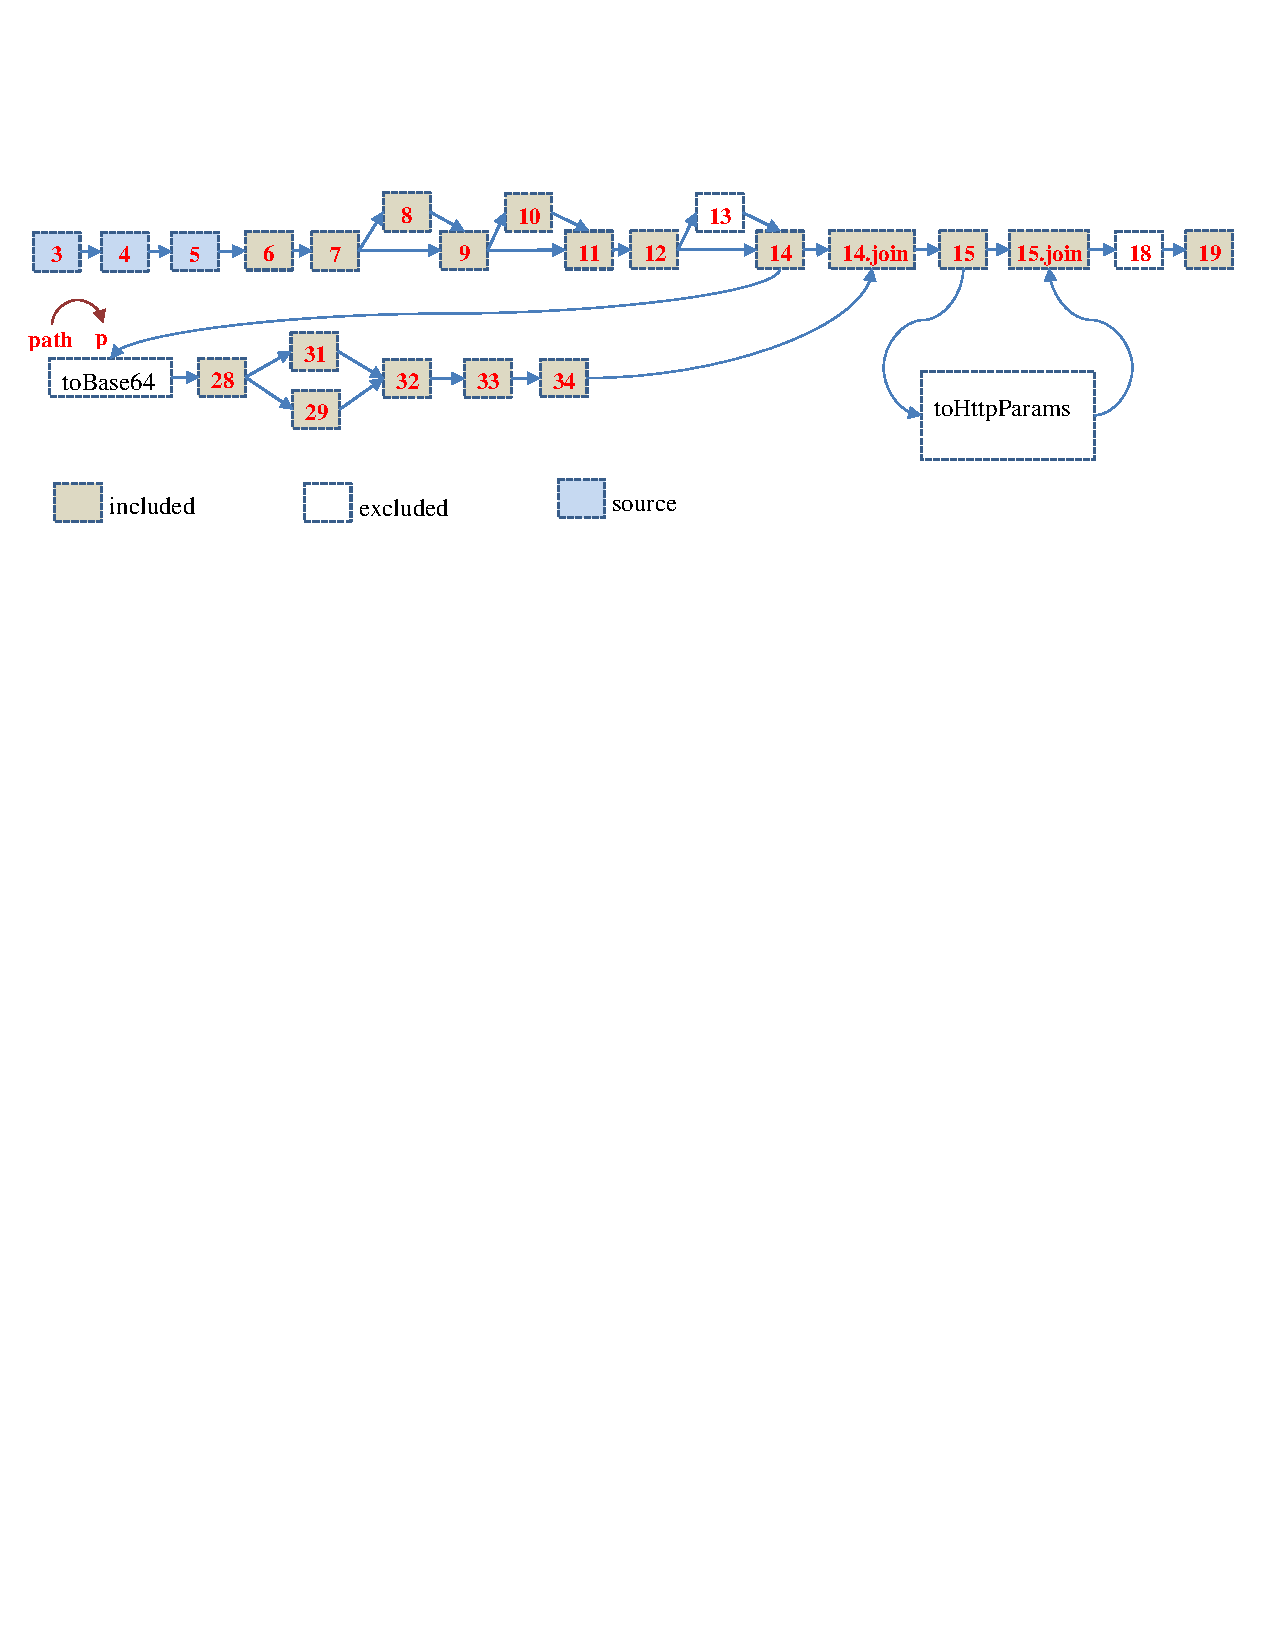
\includegraphics[width=4in]{./images/supergraph.pdf}
  \caption{Supergraph built by the analysis framework. \label{fig:supergraph}}
 \end{figure*}

\noindent
\textbf{Android application model}. An additional challenge is posed by the asynchronous nature of the Android framework and its event-guided application execution, including various callbacks. Common events are, for example, component stopping or destruction based on user-events or system-wide events, such as low memory or battery power. This execution model poses challenges in the determination of all the possible paths through which data may flow, by breaking some paths into different methods, which are not connected in the supergraph.

In our approach, we consider these methods independently: as described in detail in Section~\ref{sec:implementation} we consider each statement that extracts data from an intent as a separate \textit{source} statement and do not follow possible paths across methods that cannot be linked in the supergraph. While this choice may miss some paths, we note that a large number of these event-based method calls deals with saving the state of a component and restoring it when the component is resumed. Thus, in these cases there is no loss of information about paths and variable values.

After the preliminary step of taint propagation, the data flow analysis framework proceeds to traverse the supergraph and to collect for every point in the program the paths reaching that point from the source. The supergraph traversal starts from the source statements and adds statements to each list until a fix point is reached, and no additional statements are added to any of the lists of any program point. During this traversal, the nodes that do not use tainted variables are ignored. 


\subsection{Symbolic execution} Once the data-flow analysis framework collects all the paths for every program point, symbolic execution is used to create a formula of constraints for that point. In particular, for every program point, the list of statements is consulted and every statement different from a branching statement is added as a constraint to a symbolic formula. At the end of this step, for each program point we obtain the symbolic formula $F_p$, which models the relationship between $V_I$ and its state in that program point. 

\begin{figure}[h]
  \centering
		\begin{tabular}{lll}
			$F_p$  & $\rightarrow$ & $F_{p} \vee conj \ \vert \ conj$ \\
			$conj$ & $\rightarrow$ & $(conj \wedge term)\ \vert\ term$ \\
			$term$ & $\rightarrow$ & $stat\ \vert\ \neg stat$ \\
			$stat$ & $\rightarrow$ & $statement\ \vert\ \boldmath{var} == statement$\\
			$statement$ & $\rightarrow$ & $statement\ \boldmath{+}\ single\_stat\ \vert\ single\_stat$\\
			$single\_stat$ & $\rightarrow$ & $\boldmath{var}\ \vert\ \boldmath{constant}\ \vert\ lib\_method$ \\
			$lib\_method$ & $\rightarrow$ & $\boldmath{solv\_stat}\ \vert\ \boldmath{nonsolv\_stat}$ \\
		\end{tabular}
  	\caption{Grammar of Symbolic Formula}
	\label{fig:grammar}
 \end{figure}

The syntax of the symbolic formulas used in our approach is described by the grammar listed in Figure \ref{fig:grammar}. 
In particular, the symbol $solv\_stat$ represents statements and library methods whose operations semantics can be modeled by the solver used in the exploit generation step (see Section \ref{section:kaluzaTranslation}). These include string manipulation methods (e.g., \emph{host.contains(``example.com'')}).
The symbol $nonsolv\_stat$ represents statements and library methods whose semantics cannot be modeled by the solver. Finally, $var$ represents tainted variables, $constant$ represents constant strings, while the ``$+$'' symbol represents string concatenation. For instance, the formula $F_p$ related to the sink statement on line 20 of Figure \ref{lst:example} is derived as:

\scriptsize
($host.contains("example.com") \wedge url$$==$$"http$://$"+host+"/"$)$\bigvee$ \\
(! $host.contains("example.com") \wedge url$$==$$"http$://$www.example.com/"$)
\normalsize
We note that each term in the symbolic formula represents a statement along the path, while each new path created by a branching statements is represented using a disjunction. Assignment operations in the code are modeled using equality constraints, in order to capture the equality conditions between two expressions. 

% \noindent
% \textbf{Variable name preservation}. We highlight at this point the main difference of our approach with classic symbolic execution. In classic symbolic execution, symbolic expressions are used to represent program variable values. For instance, suppose the expression $x=y+z$ is present in the program and $y$ and $z$ are the symbolic input variables. Then, all the uses of the definition of $x$ are replaced by the symbolic expression $y+z$. In our approach, however, the main goal is to join the formula $F_p$ with the exploit state $V_E$ at the point $p$. Therefore, since $V_E$ is represented in terms of the variable names at point $p$, we need to preserve the names of the variables and indeed the chain of assignments and aliasing from the source statements to point $p$. 

% To capture such aliasing relations (for instance, those that occurs between concrete arguments of method calls and formal parameters of those method definitions), we use the production of the grammar that derives the string $\boldmath{var}\ ==\ \boldmath{var}$. For instance, in our example, an aliasing relation occurs between the variables $path$ and $p$. This aliasing relation is shown in the graph in Figure \ref{fig:supergraph} by the arrow $path \rightarrow p$, and it is represented in the symbolic formula by the term $path == p$. 

% \noindent
% \textbf{Library Methods}. As previously mentioned, we consider library methods as unit statements during path computation. However, as shown by the last rule of the grammar, during symbolic execution we divide the library methods in two sets, namely \emph{solvable statements} ($solv\_stat$) and \emph{non solvable statements} ($nonsolv\_stat$). The former includes statements that manipulate strings, which the solver can deal with (e.g., \emph{host.contains(``example.com'')}), while the latter includes statements that cannot be processed by the solver (e.g., \emph{InputStream.read(p)}). This type of statements are included in the formula and the result given by the solver for the variables in the latter set will be the whole domain (*). For instance, the solver reports that the variable $bytes$ in line 32 can be anything. 

\noindent
\textbf{Loops}. One of the main issues in symbolic execution is dealing with loops. In fact, even a single loop can generate a large number of execution paths depending on different number of iterations and paths inside the loop. Since the number of loop iterations is unknown during static analysis, a common strategy is to place an upper bound over the number of times a loop is executed symbolically. In our approach, we execute each loop symbolically one time. This choice allows us to cover the loop body statements while still having an acceptable performance.




% 3) Untainted variables. These can appear only inside statements that use tainted variables as well (because we filter out all the other statements. In the end, the solution given by the solver for the untainted variables is the whole domain (*). So how do they appear in the formula?\\




%Since the second clause does not lead to a propagation of $hostname$ to the sink, the solver is
%able to generate an exploit satisfying the first constraint. The solution will be $example.com@$ where the ``$@$'' symbol stays for any %string.

%\lstset{numbers=left, basicstyle=\ttfamily\scriptsize, breaklines=true}
%\begin{lstlisting}
%$filename.contains("..") ->
%   $filename.replace("..", ".")
%$filename.length > 0
%$filename := "/data/data/com.example/public/" + $filename;
%\end{lstlisting}




\subsection{Exploit Generation}
The input the exploit generation step, is a program point $p$, the corresponding formula $F_p$ and a set of assignments representing the exploit state $V_E$. The first operation of this step is the translation of the symbolic formula $F_p$ into the solver's language. In particular, for each member of the $solv\_stat$ statements, we create a set of constraints in the language of the solver, which model the behavior of that statement (for more details about this task, see Section \ref{sec:implementation}). The members of the $unsolv\_stat$ statements are modeled with a particular operator in the solver's language that returns the whole domain of values for the variable.



%In our threat model we focus our attention on intent payloads, not on their nature or kind: we consider payload
%contents to be the unique input that a possible attacker can exploit in order to gain control of the application environment. By doing this, differently from Chex, we do not consider attack concerning sequences of Intent messages and their interaction, but we focus our efforts on a deeper analysis about the consequences of a single intent reaction of the vulnerable application.


%The input received by an application component via an intent is a set of variables, each having a range of possible values in the domain determined by the variable type. We denote a set of such variables as $I_a=\{i_{a1}, i_{a2}, ..., i_{an}\}$. Further, we call the statements of the application component where such variables are first received \textit{source} statements. In our running example in Section~\ref{sec:running-example}, lines 4 and 6 in Figure~\ref{fig:example-code} are \textit{source} statements. In addition to the set $I_a$, the application component may also use other variables, which are not input via an intent and may or may not be under the control of an attacker. For instance, variables such as device identifiers and application database data belong to this category. We denote this set of variables with $I_b=\{i_{b1}, i_{b2}, ..., i_{bn}\}$. In the following, we assume that the attacker does not control variables in the set $I_b$, even though in practice there may exist cases where the attacker may have partial control over the set $I_b$ or obtain the values those variables from the environment.
%
%Conceptually, the application component processes the input variables according to its own logic, and produces in output a new set of variables, which we denote as $O=\{o_1, o_2, ..., o_m\}$. Correspondingly, any statements in the program where data may trigger a malicious abuse will be called a \textit{sink} statements (e.g. line 14 in Figure~\ref{fig:example}.b). Using this notation, an application component can be described formally as a function $F: I_a \cup I_b \rightarrow O$.
%
%%Conceptually, the function $F$ represents both the application logic proper and eventual data validation and sanitization operations.
%%We have not started talking about paths yet. But depending on the application, several such functions may exist for the same input, because there may be different reachable sinks.
%
%In an intent-spoofing attack, the goal of an attacker is to induce an application component to produce a desired output $O_m=F(I_a \cup I_b)$ by appropriately crafting $I_a$, such that the variables in the output $O_m$ are parameters to sensitive operations (e.g. they are values of UI elements, data being sent over the network to a server, etc.).
%
%Ideally, we want to verify that, for every possible $O_m$ desired by an attacker, there is no input $I_a$ such that $F(I_a \cup I_b)=O_m$. In practice, given that there are usually multiple sinks, and multiple potential malicious output sets $O_m$ desired by an attacker, determining every possible malicious set $O_m$ for every sink is hard. However, $O_m$ is a subset of the set of all possible outputs. So we can first determine all source-to-sink paths in the application, and then compute the set of all possible outputs via symbolic evaluation (with some approximation). At this point, we can provide a ``proof of concept'' exploit, by automatically computing a malicious input string, given the desired output.

%\begin{table*}[t]
%\begin{tabular}{|l|l|l|l|}
%\hline
%\textbf{Category} & \textbf{Pattern} & \textbf{Description} & \textbf{Taint Action} \\
%\hline
%Simple  &  $var=var_t\ op ...\ op \ var_t$ & Assignment with no function calls on & $taint(var)$ \\
%   Statement      &                                & RHS and at least one tainted & \\
%                  &                                & variable on the RHS & \\
%\hline
%User-defined     &  $var=foo(var_t,...)$  & User-defined procedure on the & $ taint(formal)$,\\
%function call    &                        & RHS of an assignment.      & $(taint(var)\ if\ isTainted(return))$ \\
%\hline
%User-defined    &  $foo(var, var_t,...)$  & User-defined procedure call & taint(stmt) \&\& taint(formal)\\
%function call    &       &    & $taint(var)$\\
%\hline
%API function  & $a=api(var_t,...)$ & API procedure on the RHS of an assignment & taint(var) \\
%   call               & $api(var, var_t,...)$ & API procedure call & $taint(var)$\\
%\hline
%\end{tabular}
%\caption{Taint Policy}
%\label{tab:Taint}
%\end{table*}

%\subsection{Path Identification}
%The first task of our approach is identification of all the different paths among sources and sinks. To do so, we build a static taint analysis framework to keep track of the variables in set $I_a$ and statements affected by those variables (as they are the only ones that the attacker can affect in our threat model).
%
%We proceed as follows. A taint is introduced for each variable whose value is derived from the set of variables $I_a$, i.e. for each variable whose value is set by the get methods of the Intent class. For instance, with respect to Fig. \ref{fig:example-code}, a taint is introduced initially for each of the variables \textit{url} and \textit{path}.
%
%At this point, the taint is propagated according to the policy summarized in Table \ref{tab:Taint}, where we denote with $var$ an untainted variable, with $var_t$ a tainted variable, $taint(var)$ the taint action on a variable $var$,and with ($taint(formal)$), the tainting action on a formal parameter of a function definition. For brevity, we report only the cases in which the taints are propagated.
%
%%TODO how do we support the assertion that the APIs are safe?
%As shown in Table \ref{tab:Taint}, the variables appearing on the LHS of an assignment containing no function calls are tainted if there exists at least a tainted variable on the RHS of that assignment. For user-defined functions having tainted variables as arguments, we propagate the taint to the corresponding formal parameter ($taint(formal)$) and taint the variable on the LHS of the assignment if the return value of the function is tainted.
%If, however, an untainted variable is passed as input to the function and tainted inside that function, that taint is preserved after exiting the function. Finally, for API function calls, we do not propagate the taints inside the functions' body, based on an assumption that they are generally safe, and also for performance reasons, which will be discussed in Section \ref{sec:implementation}. However, we make the conservative assumption that eventual untainted variables will be affected by the function call, and taint them.
%
%Taint propagation proceeds along the interprocedural control flow graph of a component and stops when a \textit{sink} statement is reached. Currently, sink statements are defined manually, and include calls to API procedures that deal with setting the values of UI elements and sending data over the network.
%
%At the end of taint analysis, the variables of an application component are partitioned into two sets: those whose values and execution may be potentially affected by the attacker's input, and those whose values and execution are not affected by an attacker's input. In addition, the statements are also partitioned into two similar sets: those statements that contain tainted variables and those statements that do not contain tainted variables. Intuitively, the execution of the former can be potentially affected by an attacker's malicious input, while execution of the latter cannot be affected by an attacker's input.
%
%\subsection{Path Computations}
%
%The described taint propagation is only the first step towards characterizing a component as a function $F$. To derive a model about the possible outputs at the sinks, we use symbolic execution over the paths discovered by the taint analysis step and employing the variables in $I_a$ as symbolic values.
%
%
%One of the main challenges of symbolic execution is \textit{path explosion}, where the paths to be considered may increase exponentially. An additional  challenge is represented by the presence of procedures, each of which defines a new execution context with its own control flow graph. Similarly to the taint analysis, in the presence of procedures, a symbolic execution framework must solve additional problems, such as variables with the same name defined in different contexts, correspondence between actual arguments of a procedure call and formal parameters of a procedure definition, and the relationship between values returned by the callee and variables of the caller.
%
%All the above challenges are exacerbated by the presence of calls to the framework APIs. In fact, due to their size and interconnectedness, the number of paths can rise very rapidly, and the complex patterns between arguments, formal parameters, and return values contribute to render symbolic execution intractable.
%
%To be able to symbolically execute the program across procedures, we construct a control flow super-graph that combines the control flow graphs of the those procedures and establishes relations between call arguments and formal parameters and between callee return values and variables at the caller site.
%In addition, to address the path explosion, in constructing this super-graph we make the following choices: 1) we prune the graph from the untainted statements and 2) similarly to taint analysis, we treat API calls as atomic instructions and do not expand them further. The former choice allows us to reduce the size of the graph, while preserving the precision of the symbolic execution as much as possible. For instance, the statement at line 6 in Fig. \ref{fig:example-code}, which is not tainted, is removed from the super-graph.
%The latter choice forces us to obtain only approximate results.
%
%After the reduced super-graph is obtained, we traverse it starting from the \textit{source statements} and, for every statement, add a term to a symbolic formula, which represents the computations on the variables of $I_a$ (See Section \ref{sec:implementation}).
%
%In general, tainted statements contain also untainted variables whose values cannot be affected by the variables in the input set $I_a$. For instance, the line 7 of the code in Fig. \ref{fig:example-code} contains a call to a user-defined procedure that has the untainted variable $user\_id$ as argument. In our approach, we include these variables in the formula. In fact, when the formula is solved, the values of these variables will be the entire domain.
%
%The symbolic execution stops when a \textit{sink} statement is encountered. For each sink, we therefore produce several conjunctive formulas, each corresponding to a computation path from a \textit{source} statement to a \textit{sink statement}. These formulas represent effectively the function $F$, which models the values computed at the sink statements starting from the variables in the input set $I_a$.
%
%\subsection{Exploit Generation}
%
%Once a symbolic formula $F$ representing the constraints and computations along a path is obtained, the next step in our approach is to attempt to generate an exploit using $F$. In fact, the existence of a path does not imply a vulnerability, since the path may contain validation and sanitization checks. Therefore, we attempt to generate an exploit in order to test for, and provide the proof of, the existence of an actual vulnerability.
%
%To generate an exploit, we use a two-step strategy. First, we use a constraint solver to solve the formula $F$ for a path without any constraints over the output variables at the sinks. In other words, we ask the solver to provide all of the input values that produce any output at all. Guided by these first results, we augment the symbolic formula with constraints that restrict the output values to a malicious set $O_m$. The solution to this augmented formula contains the set $I_a$ of malicious input values.
%
%% \subsection{Assumptions and limitations}
%
%% % TODO maybe this should be merged back somewhere else
%% In our approach has a few limitations and simplifying assumptions. First, our current implementation deals only with string variables and string operations. However, from our experience, most of the intent data carry string variables. Also, this is an implementation issue, our approach can be extended to handle other types of data.
